% ==================================================
% فصل ترجمه مقاله Nature
% ==================================================

\chapter{ترجمه فارسی مقاله \textit{Observation of constructive interference at the edge of quantum ergodicity}}
\label{chap:otoc-translation}

% مسیر تصاویر (در صورتی که فایل‌ها در پوشه `figs/` قرار داشته باشند)
\graphicspath{{figs/}}

در این جا، ترجمه‌ای تحلیلی از مقالهٔ جدید گروه \lr{Google Quantum AI} با عنوان «\lr{Observation of constructive interference at the edge of quantum ergodicity}» که در مجلهٔ \lr{Nature} در اکتبر 2025 منتشر شده است ارائه می‌شود \cite{google2025observation}. این مقاله به بررسی دینامیک سیستم‌های چندجسمی کوانتومی با استفاده از توابع همبستگی خارج از ترتیب زمانی \lr{Out-of‑Time‑Order Correlators – OTOC} پرداخته و نشان می‌دهد که اندازه‌گیری‌های مرتبهٔ دوم این تابع، اطلاعاتی را در اختیار قرار می‌دهد که در روش‌های کلاسیکی قابل دسترسی نیستند.

%============
\section{مشاهده‌ی تداخل سازنده در مرز ارگودیسیتی کوانتومی}
\label{sec:intro}

پویایی سامانه‌های چندذره‌ای کوانتومی با مشاهده‌گرهایی مشخص می‌شود که از توابع همبستگی میان نقاط متفاوت فضا و زمان بازسازی می‌شوند. در سیستم‌هایی که در آن‌ها درهم‌تنیدگی به‌سرعت رشد می‌کند، مشاهده‌گرهای کوانتومی معمولاً در زمان‌های طولانی نسبت به جزئیات دینامیک زیرین بی‌حس می‌شوند؛ این پدیده ناشی از «آشفتگی» یا همان \lr{scrambling} اطلاعات کوانتومی است. 

برای دور زدن این محدودیت و دسترسی به دینامیک مؤثر، در سال‌های اخیر از **پروتکل‌های معکوس زمانی** (\lr{time-reversal protocols}) استفاده شده است. در این پژوهش، ما با استفاده از پردازنده‌ی کوانتومی ابررسانا، **همبستگی‌های مرتبه‌دوم خارج از ترتیب زمانی** یا \lr{OTOC(2)} را به‌صورت تجربی اندازه‌گیری کردیم. نتایج نشان می‌دهند که این کمیت در مقیاس‌های زمانی طولانی همچنان به دینامیک زیرین حساس باقی می‌ماند. 

همچنین، \lr{OTOC(2)} ساختارهای همبستگی کوانتومی را در سامانه‌ای بسیار درهم‌تنیده آشکار می‌کند که بدون بهره‌گیری از تکنیک‌های معکوس زمان قابل‌دسترسی نیستند. ما این پدیده را از طریق پروتکلی آزمایشی نشان می‌دهیم که در آن، فاز رشته‌های پائولی در تصویر هایزنبرگ با درج اپراتورهای پائولی در حین تکامل کوانتومی تصادفی‌سازی می‌شود. مقادیر اندازه‌گیری‌شده‌ی \lr{OTOC(2)} تغییر قابل‌توجهی نسبت به حالت عادی نشان می‌دهند، که این امر حاکی از **تداخل سازنده میان رشته‌های پائولی** است؛ رشته‌هایی که مسیرهای حلقوی بزرگی را در فضای پیکربندی تشکیل می‌دهند.

این مکانیزم تداخل مشاهده‌شده نه‌تنها منشأ حساسیت بیشتر \lr{OTOC(2)} به دینامیک کوانتومی است، بلکه **پیچیدگی شبیه‌سازی کلاسیکی بالایی** نیز به آن می‌بخشد. ترکیب این دو ویژگی—یعنی حساسیت زیاد و دشواری شبیه‌سازی کلاسیکی—نشان می‌دهد که اندازه‌گیری \lr{OTOC(2)} می‌تواند راهی عملی به‌سوی **مزیت کوانتومی کاربردی** باشد.

در چارچوب کلی‌تر، هدف ما شناسایی و تحلیل همبستگی‌های پیچیده میان درجات آزادی بسیار زیاد در یک سامانه‌ی کوانتومی است—که موضوعی بنیادین در شبیه‌سازی دینامیک کوانتومی محسوب می‌شود. حتی مسائل طیف‌سنجی نیز را می‌توان بر پایه‌ی چند‌نقطه‌ای از همین توابع همبستگی زمان–مکان بازنویسی کرد. اما با رشد درهم‌تنیدگی، سامانه به‌طور مؤثر به حالت ارگودیک میل می‌کند و حساسیت مشاهده‌گرهای معمولی نسبت به جزئیات دینامیک به‌صورت نمایی کاهش می‌یابد. این ویژگی، تحلیل و آشکارسازی همبستگی‌های چندبدنه‌ای را در عمل بسیار دشوار می‌کند.

روش‌های کلاسیکی تحلیل آشفتگی—مانند مطالعه‌ی حساسیت به شرایط اولیه یا «اثر پروانه‌ای»—در اینجا بی‌فایده‌اند، زیرا خطی بودن معادله‌ی شرودینگر اجازه‌ی چنین رویکردهایی را نمی‌دهد. در عوض، پروتکل‌هایی که از **بازتاب یا بازآوایی زمان** (\lr{echoing}) برای حذف بخش عمده‌ای از تکامل سامانه استفاده می‌کنند، ابزار حیاتی در کاوش دینامیک‌های درهم‌تنیده شده‌اند. این روش‌ها نه‌تنها در مترو‌لوجی و سنجش کوانتومی بلکه در مطالعات مربوط به **آشوب، سیاه‌چاله‌ها و گرمایش کوانتومی** نیز نقشی کلیدی ایفا کرده‌اند.

در چارچوب تصویر هایزنبرگ، دنباله‌های دینامیکی شامل معکوس زمان را می‌توان به‌صورت **پدیده‌ی تداخل میان مسیرهای چندبدنه‌ای** در نظر گرفت. هر مرحله‌ی معکوس زمان، در واقع به افزایش بازوهای تداخلی و ترکیب‌های متقاطع جدید میان مسیرها منجر می‌شود که در نهایت در قالب کمیت‌هایی به نام \lr{OTOC} ظاهر می‌شوند. 

بنابراین، اندازه‌گیری‌های \lr{OTOC(k)} را می‌توان به‌منزله‌ی آزمایش‌های تداخل زمانی کوانتومی دانست که در آن، تعداد بازوهای تداخل (مرتبه‌ی k) تعیین‌کننده‌ی میزان دقت و عمق آشکارسازی همبستگی‌های پنهان است. در این تحقیق نشان داده می‌شود که هرچه مرتبه‌ی \lr{OTOC(k)} بالاتر باشد، حساسیت آن به دینامیک میکروسکوپی نیز افزایش می‌یابد، و به‌ویژه \lr{OTOC(2)} تداخل سازنده‌ای میان رشته‌های پائولی ایجاد می‌کند که در مشاهده‌گرهای مرتبه‌ پایین‌تر قابل‌تشخیص نیست.


%=======================
\section{حساسیت \lr{OTOCs} نسبت به دینامیک کوانتومی}
\label{sec:sensitivity}

برای درک بهتر نحوه‌ی بازیابی حساسیت به جزئیات دینامیک کوانتومی از طریق پروتکل‌های معکوس زمان، اندازه‌گیری عملگر پائولی 
\( M \in \{X,\, Y,\, Z\} \) 
روی کیوبیت \( q_m \) را در نظر می‌گیریم؛ سامانه‌ای که روی یک شبکه‌ی مربعی از کیوبیت‌ها قرار دارد و در آغاز در یکی از حالت‌های ویژه‌ی \( M \) آماده‌سازی شده است. 

اندازه‌گیری این عملگر در زمان \( t \) معادل محاسبه‌ی **همبستگی زمان‌مرتب** (Time-Ordered Correlator یا TOC) است:
\[
\langle M(t) M \rangle, \quad M(t) = U^\dagger(t) M U(t),
\]
که در آن \( U(t) \) تکامل زمانی چند‌بدنه‌ی سامانه و \( \langle \cdot \rangle \) امیدریاضی بر حالت اولیه است.  
مطابق با آزمایش‌های پیشین \cite{Kaufman2016, Zhang2023}, مقدار \(\langle M(t) M \rangle\) با گذشت زمان به‌صورت نمایی کاهش می‌یابد؛ چراکه اطلاعات کوانتومی اولیه‌ی کیوبیت \( q_m \) در فضای هیلبرت نمایی بزرگ سامانه پخش می‌شود (پدیده‌ی اسکرَملینگ).

اما این کاهش را می‌توان به‌صورت جزئی بازآوایی کرد. برای این منظور، تکامل \( U(t) \) با دنباله‌ای موسوم به **دنباله‌ی آونگ تودرتو** (\lr{nested echo sequence}) جایگزین می‌شود:
\[
U_k(t) = B(t) [M B(t)]^{k-1}, \quad B(t) = U^\dagger(t) B U(t),
\]
که در آن \( B \) یک اپراتور پائولی دیگر است که روی کیوبیت \( q_b \) (در فاصله‌ای از \( q_m \)) عمل می‌کند و \( k \ge 1 \) مرتبه‌ی تکرار بازآوایی است.  
تأثیر این دنباله را می‌توان چنین توصیف کرد: اطلاعاتی که توسط \( M \) تزریق می‌شود، با \( B \) اصلاح می‌گردد، سپس به حالت اولیه بازگردانده می‌شود، و این فرایند \( k-1 \) بار تکرار می‌گردد.

در این حالت، امیدریاضی مربوط به مشاهده‌گر نهایی (که در این کار با نماد \( C^{(2)}_k \) نمایش داده می‌شود) به‌شکل زیر نوشته می‌شود:
\[
C^{(2)}_k = \langle U_k^\dagger(t)\, M\, U_k(t)\, M \rangle.
\tag{1}
\]
این کمیت همان **همبستگی خارج از ترتیب زمانی مرتبه‌ی دوم** (\lr{OTOC(2)}) است. در نتیجه، \( C^{(2)}_k \) را می‌توان به‌طور کلی‌تر \(\mathrm{OTOC(k)}\) یا \textit{همبستگی مرتبه‌ی k} نامید.

---

\subsection{تفسیر فیزیکی معادله (1)}

رابطه‌ی (1) دو بینش مهم ارائه می‌دهد:

1. **موج‌پیشانی اطلاعات:**  
اگر اطلاعاتی که از \( q_m \) منشأ می‌گیرد هنوز به \( q_b \) نرسیده باشد، اپراتورهای \( M \) و \( B(t) \) با هم جابجایی‌پذیرند، و مقدار \( C^{(2)}_k \) برابر با مقدار اولیه‌اش باقی می‌ماند.  
در نتیجه، مرزی زمانی–فضایی به‌صورت یک «جبهه‌ی اطلاعات» (\lr{information front}) شکل می‌گیرد که سرعت گسترش درهم‌تنیدگی را نشان می‌دهد.

2. **تداخل چندمسیر در فضای پائولی:**  
اگر \( U \) از نوع کلیفورد نباشد، اطلاعات منتقل‌شده از \( M \) می‌تواند از مسیرهای مختلفی در فضای پیکربندی بازگردد. همبستگی میان رشته‌های پائولی در \( B(t) \) می‌تواند موجب **تداخل سازنده میان مسیرهای مختلف** شود؛ اثری که تنها برای \( k \ge 2 \) در \lr{OTOC(k)} ظاهر می‌شود.

---

\subsection{آزمایش‌های تجربی}

در این پژوهش برای بررسی حساسیت \lr{OTOC(2)} به جزئیات میکروسکوپی دینامیک، از مدارهای کوانتومی تصادفی متشکل از دروازه‌های تک‌کیوبیتی تصادفی و دوکیوبیتی ثابت استفاده شده است (شکل~\ref{fig2}).  
در هر آزمایش، کیوبیت‌های \( q_m \) و \( q_b \) ثابت‌اند، اما پارامترهای تصادفی دروازه‌های تک‌کیوبیتی تغییر داده می‌شوند تا مجموعه‌ای از نمونه‌های آماری به‌دست آید.

برای هر طول مدار زمانی \( t \)، مقدار \( C^{(2)}_k(q_m, q_b, t) \) بارها اندازه‌گیری شد تا نویز آماری کمتر از ۱۰٪ میانگین باشد.  
این فرآیند برای ترکیب‌های مختلفی از \( t \)، \( q_m \) و \( q_b \) و برای ۵۰ تا ۲۵۰ نمونه‌ی تصادفی تکرار گردید.  
در نهایت، تمام مقادیر آزمایشگاهی \( C^{(2)} \) و \( C^{(4)} \) با ضریب بازنرمال‌سازی یکسان (به‌دست‌آمده از استراتژی‌های کاهش خطا) مقیاس‌دهی شدند.

نتایج (در شکل~\ref{fig2}b) نشان می‌دهد که جبهه‌ی اطلاعاتی یادشده به‌وضوح قابل مشاهده است. برای هر چرخه‌ی زمانی، مرزی مشخص برای کیوبیت \( q_b \) وجود دارد که ورای آن \( C^{(4)} \approx 1 \) است. این مرز همان «مخروط نوری» سامانه است که نشان‌دهنده‌ی مجموعه‌ی کیوبیت‌هایی است که با \( q_m \) درهم‌تنیده شده‌اند.

همچنین مشاهده شد که نوسانات مدار‌به‌مدار مقدار \( C^{(4)} \)، یعنی انحراف معیار \(\sigma\) بین نمونه‌های تصادفی، در همان مرتبه‌ی بزرگی مقدار میانگین آن در نزدیکی جبهه‌ی اطلاعات است. این نتیجه تأییدی است بر اینکه \( C^{(4)} \) به‌شدت به جزئیات دینامیک زیرین \( U \) حساس است — خاصیتی که در ادامه برای یادگیری همیلتونی به‌کار گرفته می‌شود.

---

\subsection{رفتار زمانی نوسانات}

برای بررسی دقیق‌تر کاهش حساسیت در طول زمان، انحراف معیار کمیت‌های مختلفی ازجمله \(\mathrm{TOC}\)، \(\mathrm{OTOC(2)}\)، \(\mathrm{OTOC(4)}\) و مؤلفه‌ی خارج‌قطری \(\mathrm{OTOC(2)}_{\text{off-diag}}\) اندازه‌گیری شد (شکل~\ref{fig2}c).  
نتایج نشان دادند که در حالی‌که انحراف معیار TOC به‌صورت نمایی افت می‌کند و در حدود \(t = 9\) به کمتر از ۰٫۰۱ می‌رسد، نوسانات \lr{OTOCs} به‌صورت **قانون توانی** کاهش می‌یابند و حتی تا \(t = 20\) بزرگ‌تر از ۰٫۰۱ باقی می‌مانند.

این تضاد چشمگیر میان رفتار TOC و OTOC نشان می‌دهد که ساختار تداخلی OTOCها نقش اصلی را در حفظ حساسیت آن‌ها نسبت به جزئیات دینامیک کوانتومی ایفا می‌کند.

---

\subsection{نتیجه‌گیری بخش دوم}

بنابراین، \lr{OTOC(2)} و \lr{OTOC(4)} را می‌توان ابزارهایی دانست که نه‌تنها قادر به تشخیص ناحیه‌های فعال اطلاعاتی در شبکه‌ی کوانتومی هستند، بلکه حتی در حضور آشفتگی و نویز، نسبت به ساختار میکروسکوپی دینامیک نیز حساس باقی می‌مانند. این ویژگی پایه‌ی نظری نتایج بعدی مقاله است، جایی‌که نشان داده می‌شود تداخل‌های چندمسیره‌ی بزرگ در \lr{OTOC(2)} منشأ پیچیدگی شبیه‌سازی کلاسیکی و مزیت بالقوه‌ی کوانتومی‌اند.
%=======================

\section{حساسیت \lr{OTOCs} نسبت به دینامیک کوانتومی}
\label{sec:sensitivity}

برای درک بهتر نحوه‌ی بازیابی حساسیت به جزئیات دینامیک کوانتومی از طریق پروتکل‌های معکوس زمان، اندازه‌گیری عملگر پائولی 
\( M \in \{X,\, Y,\, Z\} \) 
روی کیوبیت \( q_m \) را در نظر می‌گیریم؛ سامانه‌ای که روی یک شبکه‌ی مربعی از کیوبیت‌ها قرار دارد و در آغاز در یکی از حالت‌های ویژه‌ی \( M \) آماده‌سازی شده است. 

اندازه‌گیری این عملگر در زمان \( t \) معادل محاسبه‌ی **همبستگی زمان‌مرتب** (Time-Ordered Correlator یا TOC) است:
\[
\langle M(t) M \rangle, \quad M(t) = U^\dagger(t) M U(t),
\]
که در آن \( U(t) \) تکامل زمانی چند‌بدنه‌ی سامانه و \( \langle \cdot \rangle \) امیدریاضی بر حالت اولیه است.  
مطابق با آزمایش‌های پیشین \cite{Kaufman2016, Zhang2023}, مقدار \(\langle M(t) M \rangle\) با گذشت زمان به‌صورت نمایی کاهش می‌یابد؛ چراکه اطلاعات کوانتومی اولیه‌ی کیوبیت \( q_m \) در فضای هیلبرت نمایی بزرگ سامانه پخش می‌شود (پدیده‌ی اسکرَملینگ).

اما این کاهش را می‌توان به‌صورت جزئی بازآوایی کرد. برای این منظور، تکامل \( U(t) \) با دنباله‌ای موسوم به **دنباله‌ی آونگ تودرتو** (\lr{nested echo sequence}) جایگزین می‌شود:
\[
U_k(t) = B(t) [M B(t)]^{k-1}, \quad B(t) = U^\dagger(t) B U(t),
\]
که در آن \( B \) یک اپراتور پائولی دیگر است که روی کیوبیت \( q_b \) (در فاصله‌ای از \( q_m \)) عمل می‌کند و \( k \ge 1 \) مرتبه‌ی تکرار بازآوایی است.  
تأثیر این دنباله را می‌توان چنین توصیف کرد: اطلاعاتی که توسط \( M \) تزریق می‌شود، با \( B \) اصلاح می‌گردد، سپس به حالت اولیه بازگردانده می‌شود، و این فرایند \( k-1 \) بار تکرار می‌گردد.

در این حالت، امیدریاضی مربوط به مشاهده‌گر نهایی (که در این کار با نماد \( C^{(2)}_k \) نمایش داده می‌شود) به‌شکل زیر نوشته می‌شود:
\[
C^{(2)}_k = \langle U_k^\dagger(t)\, M\, U_k(t)\, M \rangle.
\tag{1}
\]
این کمیت همان **همبستگی خارج از ترتیب زمانی مرتبه‌ی دوم** (\lr{OTOC(2)}) است. در نتیجه، \( C^{(2)}_k \) را می‌توان به‌طور کلی‌تر \(\mathrm{OTOC(k)}\) یا \textit{همبستگی مرتبه‌ی k} نامید.

---

\subsection{تفسیر فیزیکی معادله (1)}

رابطه‌ی (1) دو بینش مهم ارائه می‌دهد:

1. **موج‌پیشانی اطلاعات:**  
اگر اطلاعاتی که از \( q_m \) منشأ می‌گیرد هنوز به \( q_b \) نرسیده باشد، اپراتورهای \( M \) و \( B(t) \) با هم جابجایی‌پذیرند، و مقدار \( C^{(2)}_k \) برابر با مقدار اولیه‌اش باقی می‌ماند.  
در نتیجه، مرزی زمانی–فضایی به‌صورت یک «جبهه‌ی اطلاعات» (\lr{information front}) شکل می‌گیرد که سرعت گسترش درهم‌تنیدگی را نشان می‌دهد.

2. **تداخل چندمسیر در فضای پائولی:**  
اگر \( U \) از نوع کلیفورد نباشد، اطلاعات منتقل‌شده از \( M \) می‌تواند از مسیرهای مختلفی در فضای پیکربندی بازگردد. همبستگی میان رشته‌های پائولی در \( B(t) \) می‌تواند موجب **تداخل سازنده میان مسیرهای مختلف** شود؛ اثری که تنها برای \( k \ge 2 \) در \lr{OTOC(k)} ظاهر می‌شود.

---

\subsection{آزمایش‌های تجربی}

در این پژوهش برای بررسی حساسیت \lr{OTOC(2)} به جزئیات میکروسکوپی دینامیک، از مدارهای کوانتومی تصادفی متشکل از دروازه‌های تک‌کیوبیتی تصادفی و دوکیوبیتی ثابت استفاده شده است (شکل~\ref{fig2}).  
در هر آزمایش، کیوبیت‌های \( q_m \) و \( q_b \) ثابت‌اند، اما پارامترهای تصادفی دروازه‌های تک‌کیوبیتی تغییر داده می‌شوند تا مجموعه‌ای از نمونه‌های آماری به‌دست آید.

برای هر طول مدار زمانی \( t \)، مقدار \( C^{(2)}_k(q_m, q_b, t) \) بارها اندازه‌گیری شد تا نویز آماری کمتر از ۱۰٪ میانگین باشد.  
این فرآیند برای ترکیب‌های مختلفی از \( t \)، \( q_m \) و \( q_b \) و برای ۵۰ تا ۲۵۰ نمونه‌ی تصادفی تکرار گردید.  
در نهایت، تمام مقادیر آزمایشگاهی \( C^{(2)} \) و \( C^{(4)} \) با ضریب بازنرمال‌سازی یکسان (به‌دست‌آمده از استراتژی‌های کاهش خطا) مقیاس‌دهی شدند.

نتایج (در شکل~\ref{fig2}b) نشان می‌دهد که جبهه‌ی اطلاعاتی یادشده به‌وضوح قابل مشاهده است. برای هر چرخه‌ی زمانی، مرزی مشخص برای کیوبیت \( q_b \) وجود دارد که ورای آن \( C^{(4)} \approx 1 \) است. این مرز همان «مخروط نوری» سامانه است که نشان‌دهنده‌ی مجموعه‌ی کیوبیت‌هایی است که با \( q_m \) درهم‌تنیده شده‌اند.

همچنین مشاهده شد که نوسانات مدار‌به‌مدار مقدار \( C^{(4)} \)، یعنی انحراف معیار \(\sigma\) بین نمونه‌های تصادفی، در همان مرتبه‌ی بزرگی مقدار میانگین آن در نزدیکی جبهه‌ی اطلاعات است. این نتیجه تأییدی است بر اینکه \( C^{(4)} \) به‌شدت به جزئیات دینامیک زیرین \( U \) حساس است — خاصیتی که در ادامه برای یادگیری همیلتونی به‌کار گرفته می‌شود.

---

\subsection{رفتار زمانی نوسانات}

برای بررسی دقیق‌تر کاهش حساسیت در طول زمان، انحراف معیار کمیت‌های مختلفی ازجمله \(\mathrm{TOC}\)، \(\mathrm{OTOC(2)}\)، \(\mathrm{OTOC(4)}\) و مؤلفه‌ی خارج‌قطری \(\mathrm{OTOC(2)}_{\text{off-diag}}\) اندازه‌گیری شد (شکل~\ref{fig2}c).  
نتایج نشان دادند که در حالی‌که انحراف معیار TOC به‌صورت نمایی افت می‌کند و در حدود \(t = 9\) به کمتر از ۰٫۰۱ می‌رسد، نوسانات \lr{OTOCs} به‌صورت **قانون توانی** کاهش می‌یابند و حتی تا \(t = 20\) بزرگ‌تر از ۰٫۰۱ باقی می‌مانند.

این تضاد چشمگیر میان رفتار TOC و OTOC نشان می‌دهد که ساختار تداخلی OTOCها نقش اصلی را در حفظ حساسیت آن‌ها نسبت به جزئیات دینامیک کوانتومی ایفا می‌کند.

---

\subsection{نتیجه‌گیری بخش دوم}

بنابراین، \lr{OTOC(2)} و \lr{OTOC(4)} را می‌توان ابزارهایی دانست که نه‌تنها قادر به تشخیص ناحیه‌های فعال اطلاعاتی در شبکه‌ی کوانتومی هستند، بلکه حتی در حضور آشفتگی و نویز، نسبت به ساختار میکروسکوپی دینامیک نیز حساس باقی می‌مانند. این ویژگی پایه‌ی نظری نتایج بعدی مقاله است، جایی‌که نشان داده می‌شود تداخل‌های چندمسیره‌ی بزرگ در \lr{OTOC(2)} منشأ پیچیدگی شبیه‌سازی کلاسیکی و مزیت بالقوه‌ی کوانتومی‌اند.
%=====================
\section{تداخل حلقه‌های بزرگ در \lr{OTOC(2)}}
\label{sec:large-loop}

در بخش قبل، دیدیم که کمیت‌های \lr{OTOC(k)} نسبت به جزئیات دینامیکی سامانه بسیار حساس‌اند. در این بخش نشان داده می‌شود که ریشه‌ی این حساسیت در **پدیده‌ی تداخل چندمسیره در فضای اپراتورهای پائولی** است.  
به‌طور خاص، در \lr{OTOC(2)} مسیرهایی وجود دارند که در فضای پیکربندی تشکیل «حلقه‌های بزرگ» می‌دهند و به همین دلیل اثر تداخلی آن‌ها به‌صورت سازنده آشکار می‌شود. این تداخل‌های بزرگ مستقیماً منجر به **افزایش پیچیدگی شبیه‌سازی کلاسیکی** می‌گردند.

---

\subsection{بسط اپراتورهای زمانی در فضای پائولی}

در چارچوب تصویر هایزنبرگ، اپراتور \( B(t) = U^\dagger(t) B U(t) \) را می‌توان بر حسب پایه‌ی کامل رشته‌های پائولی \(\{P_n\}\) نوشت:
\[
B(t) = \sum_{n=1}^{4^N} b_n(t) P_n,
\]
که در آن، ضرایب \(b_n(t)\) حقیقی و زمان‌وابسته‌اند و \(N\) تعداد کیوبیت‌های سامانه است.

این بسط نشان می‌دهد که با گذشت زمان، اپراتور اولیه \(B\) در فضای پائولی گسترش می‌یابد و به ترکیبی از رشته‌های چندکیوبیتی تبدیل می‌شود — پدیده‌ای که به آن **درهم‌تنیدگی اپراتوری** (\lr{operator entanglement}) گفته می‌شود.  
در مدارهایی که شامل دروازه‌های غیرکلیفورد هستند، این گسترش به‌صورت تصاعدی رخ می‌دهد و مسیرهای پائولی در فضای اپراتور شروع به شاخه‌شدن و سپس بازترکیب می‌کنند (مطابق با شکل~\ref{fig3}a).

---

\subsection{تداخل حلقه‌های کوچک و بزرگ}

دو نوع عمده‌ی تداخل در این فضا قابل‌تشخیص است:

1. **تداخل حلقه‌های کوچک (small-loop interference):**  
این نوع تداخل هنگامی رخ می‌دهد که مسیرهای پائولی مختلف در بازه‌های کوتاه زمانی با هم بازترکیب شوند. این حالت معادل تداخل موضعی میان مسیرهای نزدیک است و در هر دو کمیت \(C^{(2)}\) و \(C^{(4)}\) وجود دارد.

2. **تداخل حلقه‌های بزرگ (large-loop interference):**  
این پدیده زمانی رخ می‌دهد که ترکیب چندین مسیر پائولی در پایان تکامل زمانی تشکیل یک حلقه‌ی کامل در فضای پیکربندی دهد. در این حالت، شرط غیرصفر بودن ردیابی در رابطه‌ی زیر برقرار می‌شود:
\[
C^{(4)} = \sum_{\alpha, \beta, \gamma, \delta} c_{\alpha\beta\gamma\delta}
\operatorname{Tr}\!\left[P_\alpha P_\beta P_\gamma P_\delta\right],
\tag{2}
\]
که در آن \(c_{\alpha\beta\gamma\delta}\) ضرایب حقیقی هستند.  
برای آن‌که جمله‌ای در مجموع بالا سهم غیرصفر داشته باشد، حاصل‌ضرب چهار رشته‌ی پائولی باید برابر با همانی باشد؛ یعنی مسیرهای \(\alpha, \beta, \gamma, \delta\) باید یک حلقه‌ی بسته تشکیل دهند.

دو نوع سهم در این رابطه ظاهر می‌شود:
- **مولفه‌ی قطری (diagonal):** زمانی‌که \(\alpha=\beta\) و \(\gamma=\delta\)، که حلقه مساحت صفر دارد.  
- **مولفه‌ی خارج‌قطری (off-diagonal):** زمانی‌که هیچ‌کدام از شاخص‌ها برابر نیستند؛ این مولفه شامل حلقه‌هایی با مساحت بزرگ در فضای اپراتور است و منبع اصلی تداخل کوانتومی محسوب می‌شود.

\textbf{توضیح فیزیکی:}  
در زبان تداخلی، هر مسیر پائولی را می‌توان بازوی یک تداخل‌سنج دانست. حلقه‌های بزرگ متناظر با مسیرهایی هستند که از چند بازوی مستقل تشکیل شده‌اند و در انتها فازهای آن‌ها به‌صورت سازنده با هم جمع می‌شوند — مشابه با پدیده‌ی تداخل چندمسیره در نورشناسی کوانتومی.

---

\subsection{آزمایش درج تصادفی اپراتور پائولی}

برای بررسی تجربی نقش این تداخل‌ها، پژوهشگران در میانه‌ی تکامل زمانی \(U\) و \(U^\dagger\)، اپراتورهای تصادفی پائولی را در برخی از چرخه‌ها درج کردند (شکل~\ref{fig3}b).  
درج این اپراتورها باعث تصادفی‌شدن فاز ضرایب \(c_{\alpha\beta\gamma\delta}\) می‌شود بدون آنکه دامنه‌ی آن‌ها تغییر کند.  
از دیدگاه تداخلی، این عمل معادل با تغییر فاز در یک بازوی تداخل‌سنج است.

با مقایسه‌ی داده‌های به‌دست‌آمده از مدارهای دارای درج پائولی و بدون آن، می‌توان میزان مشارکت تداخل کوانتومی را از تغییر همبستگی‌ها استخراج کرد.  
در شکل~\ref{fig3}c، کمیت \(1-\rho\) (که \(\rho\) ضریب همبستگی پیرسون میان دو مجموعه داده است) به‌عنوان تابعی از چرخه‌ی درج پائولی نمایش داده شده است.  
نتیجه آن است که درج پائولی تغییر چشمگیری در \(C^{(4)}\) ایجاد می‌کند، در حالی‌که تأثیر آن بر \(C^{(2)}\) بسیار کمتر است؛ این موضوع تأیید می‌کند که سهم غالب در \(C^{(4)}\) ناشی از **تداخل حلقه‌های بزرگ** است.

همچنین مشاهده شد که تأثیر درج پائولی در چرخه‌های پایانی اندکی کاهش می‌یابد که می‌تواند ناشی از **دکوهرنس خارجی** و کاهش دیدپذیری تداخل باشد.

---

\subsection{ارتباط با پیچیدگی شبیه‌سازی کلاسیکی}

درک نقش تداخل‌های بزرگ برای تعیین مرز میان شبیه‌سازی کوانتومی و کلاسیکی بسیار حیاتی است.  
در این پژوهش، مقادیر تجربی \(C^{(2)}\) با نتایج به‌دست‌آمده از الگوریتم‌های شبیه‌سازی کلاسیکی مقایسه شد، از جمله **روش مونت‌کارلو کش‌شده** (\lr{Cached Monte Carlo, CMC}) و **شبکه‌های تانسوری مونت‌کارلو**.

در آزمایش‌های شامل ۴۰ کیوبیت (شکل~\ref{fig3}d)، هرچند شبیه‌سازی‌های \lr{CMC} تا حدی با داده‌های تجربی \(C^{(2)}\) منطبق بودند (با نسبت سیگنال به نویز SNR≈5 مشابه آزمایش)، اما همین الگوریتم‌ها در بازتولید مؤلفه‌ی خارج‌قطری \(C^{(4)}_{\text{off-diag}}\) شکست خوردند (SNR≈1.1 در برابر 3.9 آزمایش).  
این نتیجه نشان می‌دهد که بخش عمده‌ی اطلاعات دینامیکی در تداخل‌های بزرگ نهفته است — بخشی که برای الگوریتم‌های کلاسیکی عملاً غیرقابل دسترس است.

\textbf{توضیح تکمیلی:}  
شکست شبیه‌سازی کلاسیکی در بازتولید \(C^{(4)}_{\text{off-diag}}\) ناشی از وجود «مسئله‌ی علامت» (\lr{sign problem}) است؛ زیرا ضرایب تداخل دارای فازهای تصادفی و نوسانی هستند که در روش‌های آماری کلاسیکی میانگین‌گیری آن‌ها به‌صورت کارآمد ممکن نیست.  
این پدیده همان ویژگی است که مرز واقعی بین «رفتار کلاسیکی قابل شبیه‌سازی» و «مزیت کوانتومی» را مشخص می‌کند.

---

\subsection{جمع‌بندی بخش سوم}

بخش حاضر نشان داد که حساسیت بالای \lr{OTOC(2)} و \lr{OTOC(4)} نسبت به جزئیات میکروسکوپی، ناشی از وجود تداخل‌های چندمسیره در فضای اپراتورهای پائولی است.  
به‌ویژه، تداخل‌های حلقه‌ی بزرگ—که از ترکیب مسیرهای مستقل با فازهای تصادفی شکل می‌گیرند—منشأ **پیچیدگی شبیه‌سازی کلاسیکی و مزیت ذاتی محاسبات کوانتومی** هستند.

این درک بنیادی، در بخش‌های بعدی (شکل‌های ۴ و ۵) مبنای تحلیل رژیم‌های فراتر از شبیه‌سازی کلاسیکی و کاربرد \lr{OTOC(2)} در یادگیری همیلتونی قرار می‌گیرد.
%====================

\section{گامی به‌سوی مزیت کوانتومی کاربردی}
\label{sec:advantage}

ترکیب دو ویژگی مهم—یعنی \textbf{حساسیت بالا} و \textbf{پیچیدگی زیاد برای شبیه‌سازی کلاسیکی}—باعث می‌شود که همبستگی‌های مرتبه‌ی دوم مانند \lr{OTOC(2)} نامزد بسیار مناسبی برای دستیابی به \textbf{مزیت کوانتومی کاربردی} باشند.  
در این بخش، دو آزمایش تجربی مستقل ارائه می‌شود که اهمیت عملی این نتیجه را نشان می‌دهند:

1. اثبات اینکه \lr{OTOC(2)} را می‌توان با دقت بالا در ناحیه‌ای اندازه‌گیری کرد که برای ابررایانه‌های کلاسیکی شبیه‌سازی‌ناپذیر است؛  
2. نمایش یک مثال کاربردی از استفاده‌ی \lr{OTOC(2)} در حل یک مسئله‌ی واقعی یادگیری همیلتونی.

---

\subsection{آزمایش در رژیم فراتر از توان شبیه‌سازی کلاسیکی}

در آزمایش نخست، مقادیر \(\mathrm{OTOC(2)}_{\text{off-diag}}\) در مدارهایی با \(65\) کیوبیت اندازه‌گیری شد (شکل~\ref{fig4}a).  
در این پیکربندی، اپراتور \(B\) به‌طور هم‌زمان روی سه کیوبیت مختلف اعمال شد تا «حجم کوانتومی مؤثر» افزایش یابد—یعنی تعداد گیت‌های دوکیوبیتی‌ای که درون مخروط‌های نوری اپراتورهای \(B\) و \(M\) قرار می‌گیرند \cite{Kechedzhi2024}.  

نتایج نشان دادند که نسبت سیگنال به نویز (SNR) در محدوده‌ی \(2 \text{ تا } 3\) باقی می‌ماند، حتی با افزایش تعداد کیوبیت‌ها. این رفتار توسط مدل تجربی خطا نیز بازتولید شد و نشان داد که با وجود افزایش اندازه‌ی سامانه، افت سیگنال بسیار کند است (شکل~\ref{fig4}b).  

از سوی دیگر، هیچ‌یک از الگوریتم‌های کلاسیکی شناخته‌شده—از جمله شبکه‌های تانسوری با فشرده‌سازی بهینه—نتوانستند نتایج را با دقت مشابه بازسازی کنند.  
برآورد هزینه‌ی محاسباتی برای شبیه‌سازی همان مدارها با استفاده از ابررایانه‌ی Frontier نشان داد که محاسبه‌ی کامل \(\mathrm{OTOC(2)}_{\text{off-diag}}\) برای یک مدار ۶۵ کیوبیتی حدود \textbf{۳٫۲ سال زمان محاسباتی} نیاز دارد (شکل~\ref{fig4}c).  
این در حالی است که داده‌های تجربی متناظر در تنها \textbf{۲٫۱ ساعت} به‌دست آمدند.  
به بیان دیگر، این آزمایش اکنون در \textit{ناحیه‌ی فراتر از کلاسیک} (\lr{beyond-classical regime}) قرار دارد—مرزی که در آن شبیه‌سازی عددی کلاسیکی دیگر عملی نیست.

\textbf{توضیح فیزیکی:}  
SNR بزرگ‌تر از یک بیانگر آن است که سیگنال اندازه‌گیری‌شده با دقت کافی از نویز تفکیک می‌شود، و هنگامی‌که این شرط در سامانه‌هایی با بیش از چند ده کیوبیت برقرار باشد، سیستم عملاً به قلمرو محاسبه‌ی کوانتومی غیرقابل‌کاهش وارد شده است.

---

\subsection{کاربرد: یادگیری همیلتونی با استفاده از \lr{OTOC(2)}}

در آزمایش دوم (شکل~\ref{fig5}a)، پژوهشگران نشان دادند که می‌توان از \(\mathrm{OTOC(2)}\) برای \textbf{یادگیری همیلتونی} استفاده کرد.  
در این روش، سامانه‌ی فیزیکی مورد نظر (با همیلتونی ناشناخته) مجموعه‌ای از داده‌های تجربی \(\mathrm{OTOC(2)}\) را تولید می‌کند.  
سپس، یک شبیه‌سازی کوانتومی از همان سامانه، ولی با پارامترهای قابل تنظیم، اجرا می‌شود.  
پارامترهای همیلتونی به‌گونه‌ای تنظیم می‌شوند که داده‌های شبیه‌سازی‌شده با داده‌های واقعی بیشترین تطابق را داشته باشند.

به‌عنوان نمونه‌ی ساده، فاز \(\xi/\pi = 0.6\) مربوط به یک گیت دوکیوبیتی بین جفت خاصی از کیوبیت‌ها به‌عنوان پارامتر ناشناخته در نظر گرفته شد (شکل~\ref{fig5}b).  
با اندازه‌گیری \(\mathrm{OTOC(2)}_{\text{off-diag}}\) برای مجموعه‌ای از ۲۰ مدار تصادفی، مشخص شد که مقادیر تجربی به‌صورت نوسانی با پارامتر \(\xi\) تغییر می‌کنند و تمام منحنی‌ها در نزدیکی مقدار واقعی هدف با شبیه‌سازی‌های کلاسیکی تلاقی دارند (شکل~\ref{fig5}c).  
در نهایت، با تعریف تابع هزینه بر اساس ریشه‌ی میانگین مربعات اختلاف داده‌های شبیه‌سازی و آزمایش، کمینه‌ی این تابع دقیقاً در مقدار \(\xi = 0.6\) قرار گرفت (شکل~\ref{fig5}d).  

این نتیجه نشان می‌دهد که \(\mathrm{OTOC(2)}\) نه‌تنها شاخصی برای آشوب و درهم‌تنیدگی است، بلکه ابزاری عملی برای استخراج پارامترهای دینامیکی سامانه‌های کوانتومی واقعی نیز به‌شمار می‌رود.

---

\subsection{تفسیر و اهمیت نتایج}

نتایج بخش حاضر نشان می‌دهند که:
- \(\mathrm{OTOC(2)}\) را می‌توان با دقت بالا در ناحیه‌ای فراتر از قابلیت شبیه‌سازی کلاسیکی اندازه‌گیری کرد؛  
- این اندازه‌گیری‌ها اطلاعات فیزیکی معنادار درباره‌ی سامانه، مانند پارامترهای همیلتونی، فراهم می‌کنند؛  
- و در نهایت، الگوریتم‌های کلاسیکی فعلی حتی در تقریب‌های مونت‌کارلو یا شبکه‌های تانسوری نیز از بازتولید این کمیت‌ها عاجزند.

به‌این‌ترتیب، اندازه‌گیری \lr{OTOC(2)} گامی عملی به‌سوی تحقق مزیت کوانتومی کاربردی است، یعنی حالتی که یک پردازنده‌ی کوانتومی نه‌تنها سریع‌تر بلکه \textbf{قادر به محاسبه‌ی کمیت‌هایی است که از نظر فیزیکی معنا‌دار و از نظر کلاسیکی غیرقابل‌دسترس‌اند}.

---

\subsection{یادداشت مفهومی برای QNLP}

از دیدگاه نظری، ساختار یادگیری همیلتونی در این مقاله شباهت زیادی به فرایند آموزش مدل‌های زبانی کوانتومی دارد.  
در هر دو مورد، سامانه‌ای فیزیکی یا مفهومی داده‌هایی تولید می‌کند که ساختار تداخلی پیچیده دارند، و مدل کوانتومی دیگری تلاش می‌کند با تنظیم پارامترها (فازها، وزن‌ها یا زاویه‌ها) آن ساختار را بازسازی کند.  
به‌طور خاص، فازهای تصادفی در OTOCها را می‌توان با فازهای وابسته به برچسب‌های نحوی در جملات فارسی در مدل‌های \lr{DisCoCat} مقایسه کرد.  
بنابراین، روش یادگیری همیلتونی با \lr{OTOC(2)} می‌تواند الهام‌بخش الگوریتم‌های \textbf{یادگیری معنایی کوانتومی} در چارچوب QNLP باشد، جایی که فازهای تانسوری جمله‌ها نقش مشابهی در بازسازی معنا ایفا می‌کنند.
%======================

\section{نتیجه‌گیری و چشم‌اندازها}
\label{sec:conclusion}

در این پژوهش، ما با بهره‌گیری از پروتکل‌های معکوس زمانی و اندازه‌گیری‌های \lr{OTOC(2)}، پدیده‌ای نو را در سامانه‌های کوانتومی چندبدنه آشکار کردیم:  
\textbf{تداخل سازنده در مرز ارگودیسیتی کوانتومی.}

این پدیده نشان می‌دهد که حتی در حالتی که سامانه به‌شدت درهم‌تنیده و آشوبناک است، ساختارهای منسجم و فازهای هم‌فاز مسیرهای اپراتوری می‌توانند در مقیاس‌های زمانی بلند خود را بازآشکار کنند.  
به‌عبارت دیگر، برخلاف انتظار متداول از ارگودیسیتی—که در آن تمام اطلاعات موضعی از بین می‌رود—بخشی از اطلاعات کوانتومی در ساختارهای تداخلی مرتبه‌بالا به‌صورت نهفته باقی می‌ماند.

اندازه‌گیری \lr{OTOC(2)} و \lr{OTOC(4)} بر روی مدارهای تصادفی ۶۵ کیوبیتی نشان داد که:
- این کمیت‌ها نسبت به جزئیات میکروسکوپی دینامیک حساس‌اند؛  
- شامل مؤلفه‌هایی هستند که ناشی از تداخل حلقه‌های بزرگ در فضای پائولی‌اند؛  
- و مقدار آن‌ها در آزمایش با دقتی قابل‌مقایسه با نویز سیستم اندازه‌گیری شد، در حالی که هیچ الگوریتم کلاسیکی قادر به بازتولید نتایج نبود.

به این ترتیب، نتایج ما نه‌تنها وجود ساختارهای تداخلی منسجم در رژیم‌های آشوبناک کوانتومی را اثبات می‌کند، بلکه راهی تجربی به‌سوی تحقق \textbf{مزیت کوانتومی کاربردی} می‌گشاید—مزیتی که مبتنی بر کمیت‌های فیزیکی قابل‌مشاهده است و از صرف اندازه‌گیری سرعت یا حجم داده‌ها فراتر می‌رود.

---

\subsection{چشم‌اندازهای آینده}

ادامه‌ی این مسیر پژوهشی می‌تواند شامل موارد زیر باشد:
- توسعه‌ی پروتکل‌های تجربی برای اندازه‌گیری \lr{OTOC(k)} با مرتبه‌های بالاتر و تحلیل رفتار آن‌ها در نزدیکی گذارهای کوانتومی؛  
- استفاده از روش‌های مشابه برای شناسایی و یادگیری پارامترهای مؤثر در سامانه‌های ماده‌ی چگال یا سامانه‌های بیولوژیکی کوانتومی؛  
- و در نهایت، به‌کارگیری چارچوب \lr{OTOC}-محور در طراحی الگوریتم‌های کوانتومی جدید برای یادگیری دینامیک‌های پیچیده.

---

\subsection{ارتباط مفهومی با پردازش زبان طبیعی کوانتومی (QNLP)}

از منظر نظری، نتایج این مقاله فراتر از حوزه‌ی فیزیک‌اند.  
در مدل‌های QNLP مبتنی بر \lr{DisCoCat}، ساختار نحوی یک جمله با شبکه‌ای از تانسورها مدل می‌شود که در فضای ترکیب معنایی با هم تداخل می‌کنند.  
به‌صورت استعاری، هر مسیر معنایی در ترکیب جمله را می‌توان معادل یک مسیر پائولی در فضای اپراتور دانست.  
در این نگاه، پدیده‌ی «تداخل سازنده» در OTOC(2) می‌تواند به‌عنوان الگوی فیزیکی برای \textbf{تداخل معنایی مثبت} در پردازش زبان طبیعی کوانتومی تفسیر شود—یعنی حالتی که چند مسیر نحوی مختلف منجر به تقویت معنایی مشترک می‌شوند.

از سوی دیگر، همان‌گونه که حلقه‌های بزرگ در فضای پائولی نشان‌دهنده‌ی همبستگی‌های چندمسیره در سامانه‌ی کوانتومی‌اند، در QNLP نیز ترکیب‌های چندمسیره‌ی نحوی می‌توانند منشأ رفتارهای فراتر از کلاسیک در تفسیر جمله‌ها باشند.  
بنابراین، پژوهش حاضر می‌تواند چارچوبی فیزیکی و مفهومی برای طراحی مدل‌های زبانی کوانتومی فراهم کند که تداخل‌های معنایی را به‌صورت طبیعی و باثبات مدیریت کنند.

---

\subsection{جمع‌بندی نهایی}

پژوهش حاضر یک نمونه‌ی تجربی روشن از چگونگی ظهور مزیت کوانتومی از دل دینامیک‌های درهم‌تنیده است.  
اندازه‌گیری دقیق \lr{OTOC(2)} نشان داد که مسیرهای فازمند در فضای اپراتور، ساختارهایی فیزیکی و قابل‌مشاهده‌اند که نه‌تنها از دیدگاه بنیادی بلکه برای کاربردهای آینده در یادگیری، شبیه‌سازی، و پردازش اطلاعات کوانتومی نیز اهمیت دارند.

به‌طور خلاصه،  
\[
\text{تداخل سازنده} \;\longrightarrow\; \text{حساسیت دینامیکی بالا} \;\longrightarrow\; \text{پیچیدگی شبیه‌سازی کلاسیکی} \;\longrightarrow\; \text{مزیت کوانتومی واقعی.}
\]
این زنجیره، چارچوب مفهومی تازه‌ای را برای درک مرز میان دینامیک‌های آشوبناک و محاسبات کوانتومی کارآمد معرفی می‌کند.
%============================

\section{پتانسیل‌های پژوهشی برای پردازش زبان طبیعی کوانتومی (QNLP)}
\label{sec:qnlfuture}

\subsection{مدل‌سازی تداخل معنایی با الهام از OTOC(2)}

نتایج این مقاله نشان می‌دهند که ساختارهای تداخل سازنده در OTOC(2) منجر به بازیابی اطلاعات نهفته در سامانه‌های درهم‌تنیده می‌شوند.  
در حوزه‌ی QNLP، همین مفهوم می‌تواند برای مدل‌سازی \textbf{تداخل معنایی} میان مسیرهای نحوی و مفهومی در جملات به‌کار گرفته شود.

در چارچوب \lr{DisCoCat}، جمله به‌صورت شبکه‌ای از دیاگرام‌های مونوییدی ترکیبی نمایش داده می‌شود که مسیرهای مختلف ترکیب نحوی را به‌صورت تانسوری باهم ترکیب می‌کند. اگر هر مسیر معنایی را به یک «مسیر اپراتور» تشبیه کنیم، فازهای معنایی حاصل از برچسب‌های نحوی می‌توانند همان نقش فازهای اپراتوری در \lr{OTOC(2)} را ایفا کنند.

به‌عبارت دیگر، می‌توان یک \textbf{OTOC زبانی} تعریف کرد که حساسیت معنای جمله به تغییرات نحوی را اندازه‌گیری کند:
\[
C^{(2)}_{\text{lang}} = \langle \psi | U^\dagger M U M | \psi \rangle,
\]
که در آن \(U\) تکامل معنایی، \(M\) عملگر نحوی، و \(|\psi\rangle\) نمایش برداری جمله است.  
تحلیل رفتار این کمیت برای جملات با ساختارهای مشابه می‌تواند به تعریف کمیت‌های جدیدی برای \textbf{تداخل معنایی مثبت و منفی} در زبان طبیعی کوانتومی منجر شود.

---

\subsection{توسعه‌ی الگوریتم‌های یادگیری فازی در lambeq با الهام از یادگیری همیلتونی}

پژوهش گوگل نشان داد که می‌توان از \lr{OTOC(2)} برای یادگیری پارامترهای همیلتونی از داده‌های تجربی استفاده کرد.  
این روش را می‌توان در چارچوب \lr{lambeq} به‌صورت یک الگوریتم یادگیری فازی–کوانتومی بازنویسی کرد. در این رویکرد:

- دیاگرام‌های زبانی \lr{lambeq} به مدارهای کوانتومی تبدیل می‌شوند که پارامترهای قابل آموزش (زاویه‌ها یا فازها) دارند؛  
- مجموعه‌ای از جملات آموزشی با معانی هدف (بردارهای مفهومی) تهیه می‌شوند؛  
- سپس، با استفاده از تابع هزینه‌ای مشابه با تابع یادگیری همیلتونی،
\[
L = \sum_i \left| C^{(2)}_{\text{pred},i} - C^{(2)}_{\text{target},i} \right|^2,
\]
پارامترهای مدل به‌گونه‌ای تنظیم می‌شوند که تداخل معنایی در مدار زبانی بیشترین تطابق را با هدف داشته باشد.

به‌این‌ترتیب، روش‌های \lr{OTOC}-محور می‌توانند چارچوبی عمومی برای \textbf{آموزش تداخل‌محور مدل‌های زبانی کوانتومی} فراهم کنند—رویکردی که نه‌تنها از نظر فیزیکی بنیادین است، بلکه در سطح نظری می‌تواند رفتارهای غیرخطی و غیرارگودیک معنا را در زبان‌های طبیعی مدل کند.

---

\subsection{چشم‌انداز نظری برای مقاله‌ی آینده}

ترکیب مفاهیم OTOC با QNLP می‌تواند موضوع یک مقاله‌ی نظری مستقل با محوریت زیر باشد:
\begin{itemize}
	\item \textbf{تعریف OTOC زبانی:} معرفی کمیتی برای سنجش حساسیت معنایی جمله به تغییرات نحوی، با استفاده از مدارهای \lr{lambeq}.
	\item \textbf{شبیه‌سازی تداخل معنایی:} مدل‌سازی interference در فضای تانسوری با الهام از تداخل حلقه‌های بزرگ در OTOC(2).
	\item \textbf{یادگیری فازهای معنایی:} توسعه‌ی الگوریتمی مشابه یادگیری همیلتونی برای استخراج پارامترهای معنایی در مدل‌های زبانی کوانتومی.
	\item \textbf{تحلیل مزیت کوانتومی در QNLP:} ارزیابی این‌که کدام ساختارهای نحوی یا معنایی بیشترین پیچیدگی تداخلی را دارند و از نظر محاسباتی فراتر از مدل‌های کلاسیکی‌اند.
\end{itemize}

به‌طور خلاصه، پیوند میان \lr{OTOC(2)} و \lr{DisCoCat} می‌تواند منجر به شاخه‌ی تازه‌ای از پژوهش شود که می‌توان آن را \textbf{«دینامیک تداخلی در زبان‌شناسی کوانتومی»} (\lr{Interferential QNLP Dynamics}) نامید.
%==================
\subsection{شبیه‌سازی پروتکل‌های معکوس زمانی با Qiskit}
\label{sec:qiskit-sim}

از دیدگاه عملی، پروتکل‌های معکوس زمانی مورد استفاده در این پژوهش را می‌توان با استفاده از محیط \lr{Qiskit} شبیه‌سازی کرد.  
در این چارچوب، تکامل زمانی \( U(t) = e^{-iHt} \) و وارون آن \( U^\dagger(t) \) به‌صورت دو بلوک مجزا در مدار کوانتومی پیاده‌سازی می‌شوند.  
هر بلوک شامل دروازه‌هایی است که از تجزیه‌ی همیلتونی \(H\) به اجزای دوکیوبیتی و تک‌کیوبیتی به‌دست می‌آیند.

علاوه بر این، بسته‌ی \lr{qiskit-dynamics} امکان شبیه‌سازی مستقیم اپراتورهای همیلتونی و تکامل‌های پیوسته را فراهم می‌کند،  
در حالی که \lr{qiskit.quantum\_info} ابزارهای لازم برای محاسبه‌ی همبستگی‌های زمانی، شامل \lr{OTOC(2)}، را در اختیار می‌گذارد.

به‌این‌ترتیب، می‌توان مدارهای مربوط به معکوس زمانی مقاله را برای سامانه‌های کوچک‌تر (تا حدود ۸ یا ۱۰ کیوبیت) روی شبیه‌سازهای محلی یا بک‌اندهای کوانتومی IBM اجرا کرد و تکامل OTOC را برحسب زمان مشاهده نمود.  
این رویکرد راهی عملی برای بررسی عددی ایده‌های مقاله‌ی گوگل در محیط‌های پژوهشی مانند \lr{lambeq} و \lr{QNLP} فراهم می‌کند، جایی‌که می‌توان از همان ساختارهای مدار برای تحلیل تداخل‌های معنایی و زمانی بهره گرفت.



%++++++++++++++++++++++



\section{مقدمه و انگیزهٔ پژوهش}

دینامیک سیستم‌های چندجسمی کوانتومی غالباً با همبستگی‌هایی در مکان‌ها و زمان‌های مختلف مشخص می‌شود. در سامانه‌هایی که به سرعت درهم‌تنیده می‌شوند، بیشتر مشاهده‌پذیرهای محلی در زمان‌های طولانی به جزئیات دینامیک حساس نیستند و به بیان ساده، اطلاعات اولیه در فضای هیلبرت وسیع «پخش» یا \lr{scramble} می‌شود. این مسئله باعث می‌شود که اندازه‌گیری‌های متعارف در مدت زمان نسبتاً کوتاهی فروپاشی کرده و نتوانند آشوب کوانتومی و ارگودیسیتی را آشکار کنند.  پژوهشگران برای غلبه بر این محدودیت از پروتکل‌های زمان-معکوس یا «دنبالهٔ اکو» استفاده می‌کنند تا بخش عمدهٔ تکامل را خنثی کرده و سیگنال‌های ظریف را بازیابی کنند.
در این مقاله، تیم \lr{Google Quantum AI} خانواده‌ای از آزمایش‌های \lr{OTOC} را بر روی پردازندهٔ کوانتومی مبتنی بر کیوبیت‌های ابررسانا انجام می‌دهد. آنها با تغییر تعداد بازوهای تداخل (مرتبهٔ \(k\) تابع \lr{OTOC}) و افزودن جابجایی‌های فاز تصادفی یا منسجم، نشان می‌دهند که اندازه‌گیری \lr{OTOC(2)} نسبت به جزئیات میکروسکوپی تکامل بسیار حساس‌تر از همبستگی‌های عادی و مرتبهٔ اول است

\begin{figure}[htbp]
  \centering
  \IfFileExists{figs/fig1.png}{%
    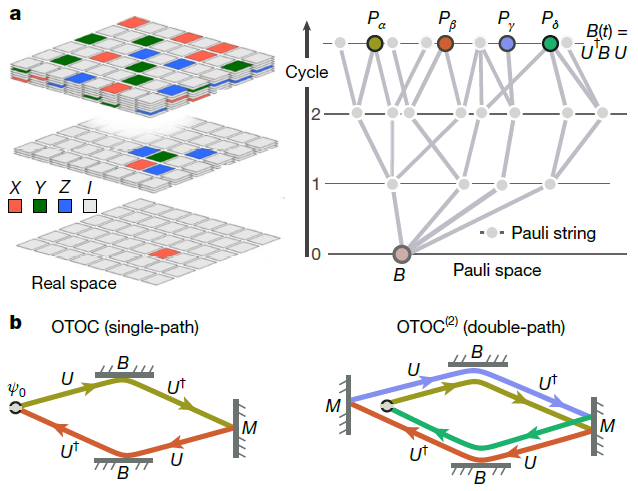
\includegraphics[width=0.85\textwidth]{figs/fig1.png}
  }{%
    \fbox{تصویر 'figs/fig1.pdf' یافت نشد؛ در صورت وجود، آن را در پوشه `figs/` قرار دهید.}
  }
  \caption{ساختار کلی و شماتیکِ پروتکل‌های OTOC (شکل توضیحی). }
  \label{fig:otoc-protocol}
\end{figure}

\section{تعریف و فرمول‌بندی \lr{OTOC}}

فرض کنید دو عملگر کوانتومی \(A\) و \(B\) را داریم. در تصویر هایزنبرگ، عملگر \(A(t)=U^{\dagger}(t)\,A\,U(t)\) با گذر زمان \(t\) تکامل می‌یابد که در آن \(U(t)=e^{-iHt}\) تکامل زمانی تحت همیلتونی \(H\) است. تابع همبستگی خارج از ترتیب زمانی \lr{OTOC} برای این دو عملگر به صورت زیر تعریف می‌شود:
\begin{equation}
  OTOC(t)=\langle A(t)\,B\,A(t)\,B\rangle,
\end{equation}
که در آن \(\langle\cdot\rangle\) میانگین روی حالت اولیهٔ سیستم است. اگر \(A\) و \(B\) در ابتدای زمان جابه‌جایی‌پذیر باشند اما با گذر زمان commute نکنند، مقدار \lr{OTOC} کاهش می‌یابد و این کاهش نشانه‌ای از پخش اطلاعات (اثر پروانه‌ای کوانتومی) است.

پژوهشگران برای دسترسی به اطلاعات دقیق‌تر، از نسخهٔ مرتبهٔ دوم \lr{OTOC(2)} استفاده کردند که با دو بار اجرای پروتکل زمان-معکوس به دست می‌آید. فرمول عمومی \lr{OTOC(k)} به صورت زیر است:
\begin{equation}
  \mathcal{C}_k^{(2)}(t)=\bigl\langle \left[ U^{\dagger}(t)\,B\,U(t)\,M\right]^k \bigr\rangle,
\end{equation}
که در آن \(M\) یک عملگر پائولی (مثلاً \(X\) یا \(Z\)) است و \(k\) تعداد بازوهای تداخل را تعیین می‌کند. برای \(k=2\) داریم
\begin{equation}
  \mathcal{C}_2^{(2)}=\langle U^{\dagger}(t)\,B\,U(t)\,M\,U^{\dagger}(t)\,B\,U(t)\,M\rangle.
\end{equation}
این کمیت همان \lr{OTOC(2)} است و می‌تواند به صورت جمعی از چهار رشتهٔ پائولی در فضای پائولی بازنویسی شود. در صورتی که حاصل ضرب چهار رشته به عملگر یکه منتهی شود، تداخل سازنده رخ می‌دهد و سهم آن مسیر تقویت می‌شود.

\section{پروتکل‌های آزمایشی و حساسیت \lr{OTOC}}

در آزمایش‌های این مقاله، پردازندهٔ کوانتومی شامل شبکه‌ای از کیوبیت‌های ابررسانا است که با گیت‌های تک‌کیوبیتی تصادفی و گیت‌های دوکیوبیتی ثابت اجرا می‌شوند. ابتدا دو کیوبیت مشخص \(q_m\) و \(q_b\) به عنوان محل اعمال عملگرهای \(M\) و \(B\) انتخاب می‌شوند. سپس مدارهای تصادفی مختلف با پارامترهای گیت‌های تک‌کیوبیتی متفاوت تولید شده و برای هر مدار، مقدار \(\mathcal{C}_k^{(2)}\) اندازه‌گیری می‌شود.
. برای کاهش نویز، اندازه‌گیری‌ها آنقدر تکرار می‌شود تا خطای آماری کمتر از ده درصد مقدار میانگین باشد.  در نهایت، تمام مقادیر با عامل مقیاس جهانی که از استراتژی‌های تصحیح خطا بدست می‌آید نرمال‌سازی می‌شوند.
نتایج نشان می‌دهد که \lr{OTOC(2)} (و به طور کلی \lr{OTOC(k)}) نسبت به جزئیات دینامیک کوانتومی حساس است. برای مثال، با اندازه‌گیری \(\mathcal{C}^{(4)}\) برای فواصل مختلف بین \(q_m\) و \(q_b\)، مرز واضحی مشاهده می‌شود که فراتر از آن مقدار \lr{OTOC} تقریباً برابر یک است؛ این مرز همان مخروط نوری کیوبیت \(q_m\) است. علاوه بر این، انحراف معیار \lr{OTOC(2)} در نزدیکی مرز اطلاعات هم‌مرتبه با مقدار متوسط آن است، که بیانگر حساسیت زیاد این تابع به تکامل زیرین است. مقایسه با همبستگی‌های ترتیب زمانی معمول نشان می‌دهد که انحراف معیار \lr{OTOC} به صورت قانون توانی آهسته فرو می‌ریزد، در حالی که همبستگی‌های عادی به سرعت نمایی کاهش می‌یابند.

\begin{figure}[htbp]
  \centering
  \IfFileExists{figs/fig2.png}{%
    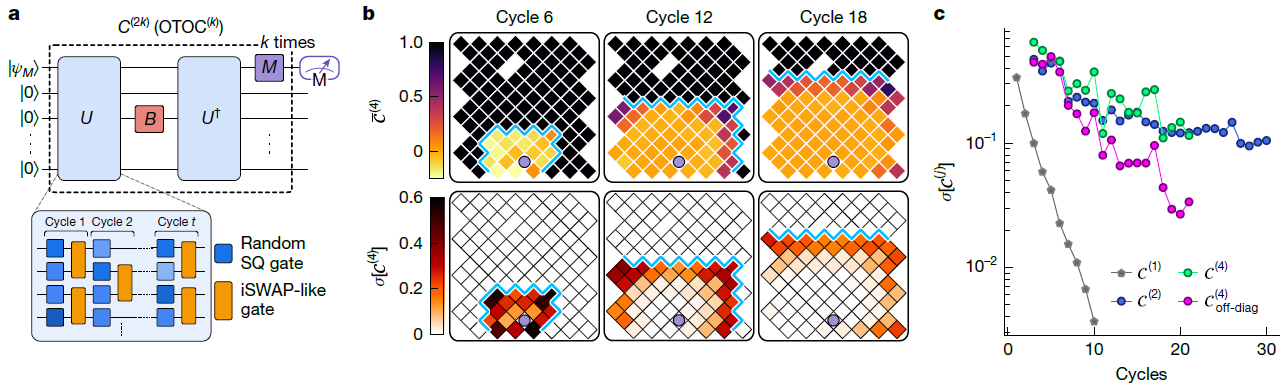
\includegraphics[width=0.8\textwidth]{figs/fig2.png}
  }{%
    \fbox{تصویر 'figs/fig2.pdf' یافت نشد؛ در صورت وجود، آن را در پوشه `figs/` قرار دهید.}
  }
  \caption{حساسیت OTOC به جزئیات میکروسکوپی دینامیک — شکلِ شماتیک/نمونه.}
  \label{fig:otoc-sensitivity}
\end{figure}

\section{تداخل بزرگ و حلقه‌های سازنده در \lr{OTOC(2)}}

در بخش دیگری از آزمایش، پژوهشگران تغییر کوچکی در فاز یکی از بازوهای تداخل ایجاد کردند تا تأثیر تداخل کوانتومی را بررسی کنند. آن‌ها نشان دادند که \lr{OTOC(2)} به این تغییرات فاز بسیار حساس است و این حساسیت به دلیل تداخل سازنده میان مسیرهای مختلف در فضای پائولی است



. در این حالت، ترکیب چهار رشتهٔ پائولی می‌تواند به عملگر یکه منجر شود و بنابراین سیگنال تقویت شود. این نوع تداخل، که به «تداخل حلقهٔ بزرگ» معروف است، در \lr{OTOC(1)} مشاهده نمی‌شود و محاسبهٔ کلاسیکی آن بسیار دشوار است. برای سیستم‌های با ۴۰ تا ۶۵ کیوبیت، شبیه‌سازی دقیق این کمیت با کامپیوترهای کلاسیک به چند سال زمان نیاز دارد، در حالی که پردازندهٔ کوانتومی می‌تواند آن را در چند ساعت اندازه‌گیری کند.

\begin{figure}[htbp]
  \centering
  \IfFileExists{figs/fig3.png}{%
    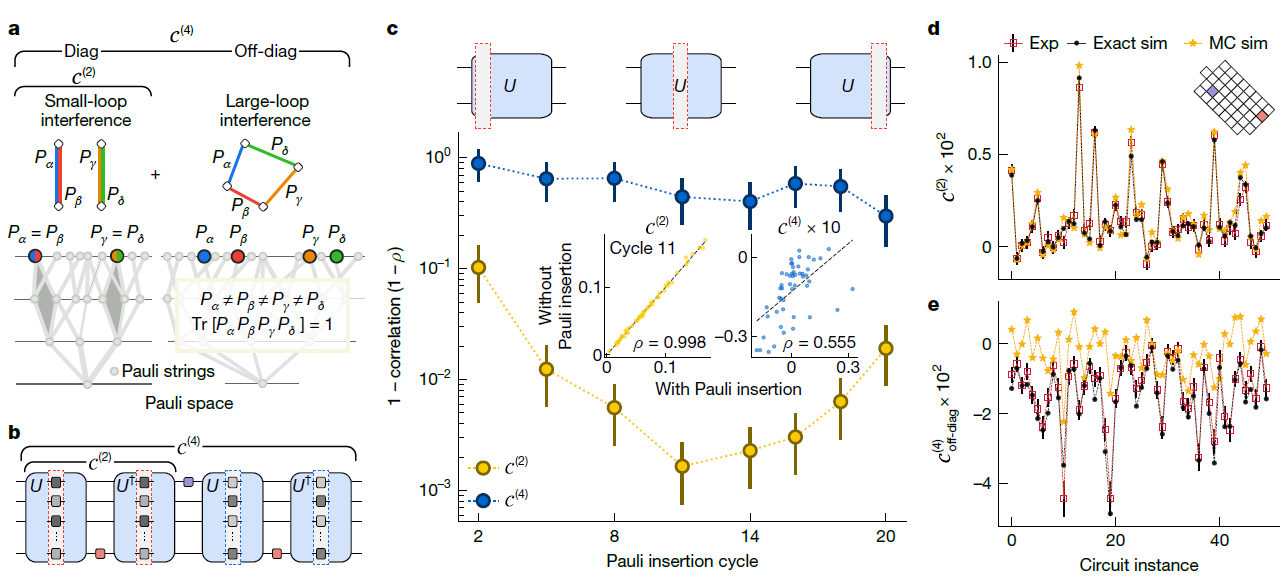
\includegraphics[width=0.75\textwidth]{figs/fig3.png}
  }{%
    \fbox{تصویر 'figs/fig3.pdf' یافت نشد؛ در صورت وجود، آن را در پوشه `figs/` قرار دهید.}
  }
  \caption{نمونه‌ای از «تداخل حلقهٔ بزرگ» که منجر به تقویت سیگنال OTOC می‌شود. }
  \label{fig:otoc-interference}
\end{figure}

\section{کاربرد در یادگیری همیلتونی}

یکی از کاربردهای مهم \lr{OTOC(2)} که در مقاله مورد بررسی قرار گرفته «یادگیری همیلتونی» است. فرض کنید سیستم فیزیکی واقعی دارای همیلتونی مجهولی با چند پارامتر ناشناخته باشد. می‌توان با اندازه‌گیری \lr{OTOC(2)} در این سیستم و مقایسهٔ آن با شبیه‌سازی کوانتومی همان سیستم (که در آن پارامترها متغیر هستند)، مقدار پارامترهای ناشناخته را پیدا کرد. پژوهشگران برای نشان دادن این مفهوم، یک مثال تک‌پارامتری را در نظر گرفتند که در آن فاز \(\xi\) یک گیت دوکیوبیتی ناشناخته است. آنها مجموعه‌ای از داده‌های \(\mathcal{C}_{\text{off-diag}}^{(4)}\) را از ۲۰ مدار تصادفی شبیه‌سازی‌شده به عنوان «داده‌های سیستم فیزیکی» در نظر گرفتند و سپس همان مدارها را روی پردازندهٔ کوانتومی اجرا کردند. با تغییر \(\xi\) و محاسبهٔ اختلاف بین داده‌های تجربی و داده‌های شبیه‌سازی‌شده، نموداری به دست آمد که حداقل آن دقیقاً برابر مقدار واقعی \(\xi\) بود. این آزمایش نشان می‌دهد که \lr{OTOC(2)} می‌تواند به عنوان ابزاری قدرتمند برای تخمین پارامترهای همیلتونی پیچیده استفاده شود.

\begin{figure}[htbp]
  \centering
  \IfFileExists{figs/fig4.png}{%
    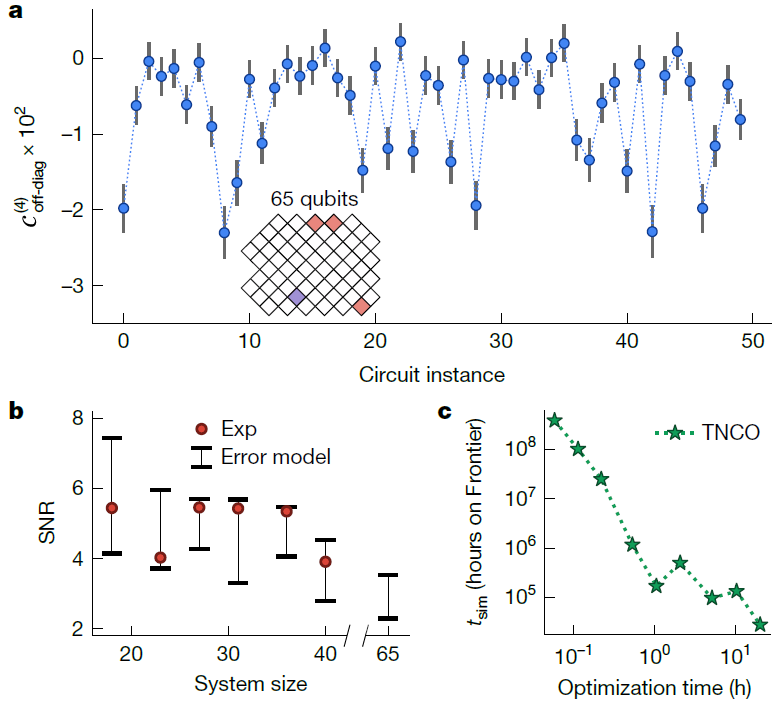
\includegraphics[width=0.8\textwidth]{figs/fig4.png}
  }{%
    \fbox{تصویر 'figs/fig5.pdf' یافت نشد؛ در صورت وجود، آن را در پوشه `figs/` قرار دهید.}
  }
  \caption{نمونه‌ای از روند به‌کارگیری OTOC در یادگیری همیلتونی؛ منحنی اختلاف یا loss بر حسب پارامتر فاز \(\xi\).}
  \label{fig:otoc-hamiltonian-learning}
\end{figure}


\begin{figure}[htbp]
	\centering
	\IfFileExists{figs/fig5.png}{%
		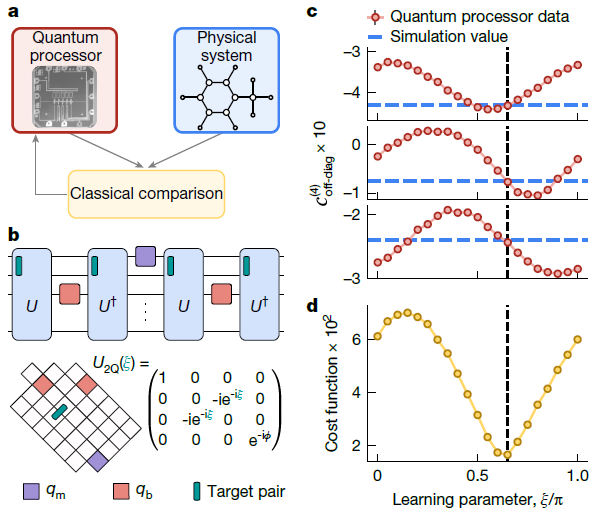
\includegraphics[width=0.8\textwidth]{figs/fig5.png}
	}{%
		\fbox{تصویر 'figs/fig5.pdf' یافت نشد؛ در صورت وجود، آن را در پوشه `figs/` قرار دهید.}
	}
	\caption{نیاز به تکیمل کپشن }
	\label{fig:otoc-hamiltonian-learning}
\end{figure}
\section{مزیت کوانتومی عملیاتی}

مقالهٔ گوگل نشان می‌دهد که \lr{OTOC(2)} نه تنها به پدیده‌های بنیادین مانند آشوب کوانتومی و تداخل سازنده حساس است، بلکه از نظر پیچیدگی محاسباتی در محدوده‌ای قرار دارد که شبیه‌سازی کلاسیکی آن فعلاً امکان‌پذیر نیست. در یک آزمایش، اندازه‌گیری \(\mathcal{C}_{\text{off-diag}}^{(4)}\) برای مدارهای ۶۵ کیوبیتی انجام شد و دقت سیگنال در حد \lr{SNR} بین ۲ تا ۳ باقی ماند

. تخمین زده شد که شبیه‌سازی همین داده‌ها با استفاده از الگوریتم‌های شبکهٔ تانسوری روی ابررایانهٔ \lr{Frontier} حدود ۳.۲ سال زمان می‌برد
، در حالی که اندازه‌گیری آزمایشی تنها ۲.۱ ساعت طول کشید. این اختلاف عظیم، همراه با قابلیت استخراج اطلاعات مفید (مانند یادگیری همیلتونی)، نشان می‌دهد که \lr{OTOC(2)} گزینهٔ مناسبی برای دستیابی به مزیت کوانتومی عملیاتی است.
\section{جمع‌بندی  }

در این فصل ترجمهٔ مختصری از مقالهٔ «مشاهدهٔ تداخل سازنده در لبهٔ ارگودیسیتی کوانتومی» ارائه شد. مقاله نشان می‌دهد که چگونه اندازه‌گیری‌های \lr{OTOC(2)} می‌توانند ساختارهای تداخلی پیچیده و حساسیت بالایی به دینامیک کوانتومی داشته باشند و در عین حال شبیه‌سازی کلاسیکی آن‌ها فوق‌العاده دشوار است. این ویژگی‌ها، همراه با کاربردهای عملی مانند یادگیری همیلتونی، راهی ملموس به سوی مزیت کوانتومی در سیستم‌های واقعی باز می‌کند.

\subsection*{اهمیت مقاله}
این کار اهمیت زیادی دارد چون نشان می‌دهد کمیت‌هایی مانند \lr{OTOC(2)} می‌توانند اطلاعاتی بنیادین دربارهٔ آشوب و پخش اطلاعات در سامانه‌های چندجسمی ارائه دهند که با ابزارهای متعارف قابل دسترسی نیست. همچنین نشان داده شد که اندازه‌گیری‌های انتخاب‌شده روی سخت‌افزار کوانتومی واقعی در مقیاس‌هایی که شبیه‌سازی آن‌ها کلاسیکی دشوار است، عملی و نسبتاً سریع است.

\subsection*{نوآوری‌های کلیدی}
نوآوری‌های اصلی مقاله را می‌توان به طور خلاصه این‌گونه بیان کرد:
\begin{itemize}
  \item معرفی و مطالعهٔ سیستماتیک \lr{OTOC(2)} و کاربرد آن برای آشکارسازی تداخل سازنده در مسیرهای تکاملی مختلف.
  \item طراحی پروتکل‌های زمان-معکوس و استفاده از دستکاری فاز و تعداد بازوهای تداخل برای تقویت سیگنال‌های ظریف کوانتومی.
  \item ارائهٔ شواهد تجربی از محدوده‌ای که در آن اندازه‌گیری‌های خاص روی سخت‌افزار کوانتومی می‌توانند مزیت زمانی نسبت به شبیه‌سازی کلاسیکی داشته باشند (نمونهٔ عملی از مزیت کوانتومی عملیاتی).
\end{itemize}

\subsection*{کاربردهای احتمالی}
نتایج این پژوهش چند کاربرد بالقوه را پیش‌روی پژوهشگران می‌گذارد:
\begin{itemize}
  \item یادگیری همیلتونی: استفاده از \lr{OTOC(2)} به عنوان معیار کمّی برای برازش پارامترهای همیلتونی سامانه‌های چندجسمی که شبیه‌سازی آن‌ها کلاسیکی دشوار است.
  \item تشخیص و تحلیل آشوب کوانتومی و انتقال‌های دینامیکی: حساسیت بالای این کمیت می‌تواند برای شناسایی گذارهای دینامیکی و نقاط بحرانی مفید باشد.
  \item سنجش و اعتبارسنجی سخت‌افزار کوانتومی در مقیاس‌های بزرگ: اندازه‌گیری‌هایی که شبیه‌سازی آن‌ها برای کامپیوترهای کلاسیک زمان‌بر است، می‌تواند معیاری برای سنجش توان حقیقی سیستم باشد.
  \item کاربردهای سنجشی  \lr{(quantum sensing)}: طراحی پروتکل‌هایی که از تداخل سازنده برای تقویت سیگنال‌های ضعیف استفاده کنند.
\end{itemize}

\subsection*{محدودیت‌ها و چشم‌اندازها}
چند محدودیت مهم نیز باید مدنظر باشد: نیاز به کنترل نویز و خطا در گیت‌ها برای مقیاس‌های بزرگ‌تر، وابستگی نتایج به انتخاب دقیق مدارها و عملگرها، و نیاز به آمار زیاد برای کاهش خطای آماری. چشم‌اندازهای آینده شامل بهبود روش‌های تصحیح خطا، بهینه‌سازی طراحی مدارها برای افزایش SNR، و تعمیم مفاهیم به کلاس‌های گسترده‌تر همیلتونی‌ها و نشانه‌ها است.
